\section{Synchronization (PPT+PPS)}
\gls{ptp} synchronization is utilized to synchronize the two cameras.
To verify the synchronization, the cameras were configured to pull the \textit{Line 2} \gls{gpio} pin high during the active exposure period, as indicated in Table \ref{tab:triton_pinout}.
This signal was then connected to an oscilloscope to measure the synchronization offset, which represents the time difference between the two cameras, as shown in Figure \ref{fig:sync_offset}.

In most cases, the synchronization offset varied between $\pm20\mu s$, but occasionally reached as high as $\pm50\mu s$.
Nevertheless, these values are within the acceptable range, as they are significantly lower than the exposure time, even when operating in daylight conditions.

The cameras also report their estimated \gls{ptp} offset, which partially aligned with the measured offset, but was not totally accurate.

\begin{table}
    \centering
    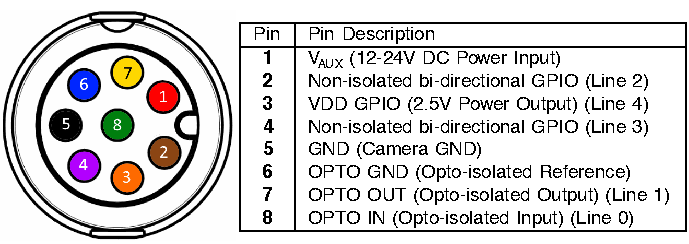
\includegraphics[width=\textwidth]{figures/triton_pinout.pdf}
    \caption{\cam \gls{gpio} connector \cite{lucidvisionlabsTritonMPPolarized2020}}
    \label{tab:triton_pinout}
\end{table}

\subsection{Reduce trigger latency}
It is possible to reduce the trigger latency of the cameras, which results in a lower synchronization offset.
This can be achieved by setting the \code{TriggerLatency} node to \code{OneLine}.
This reduces the average trigger offset down to $10\mu s$.
Unfortunately, this option becomes unavailable while the \code{TriggerOverlap} node is set to \code{set_PreviousFrame}, which is required to reach higher framerates.

\begin{figure}[H]
    \centering
    \subcaptionbox{Synchronization at $25ms$ resolution.
        \label{fig:sync_25us}}{
        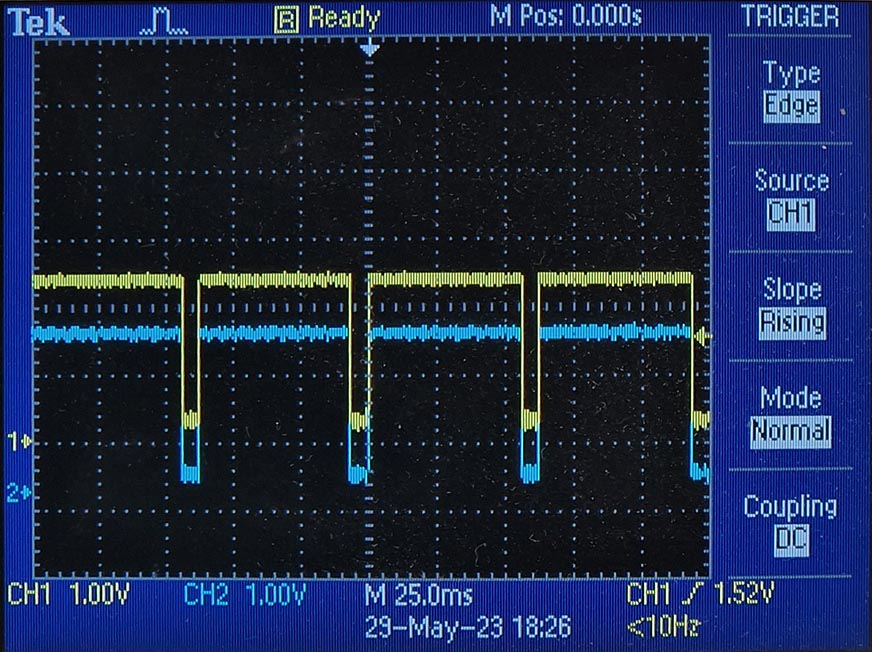
\includegraphics[width=0.8\textwidth]{figures/synchronization/ms.jpg}
    }
    \subcaptionbox{Synchronization at $10\mu s$ resolution.}{
        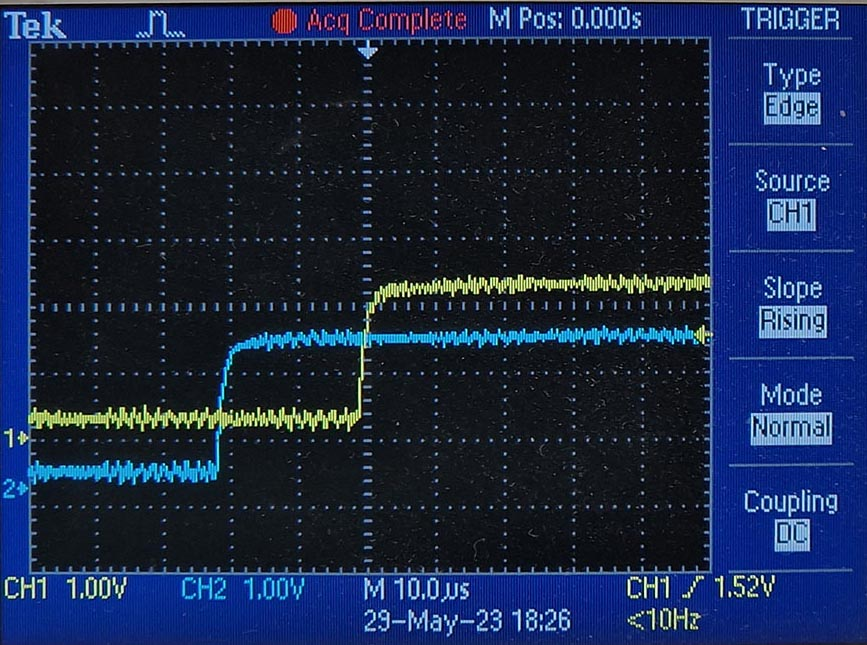
\includegraphics[width=0.8\textwidth]{figures/synchronization/us.jpg}
    }
    \caption{Measured synchronization offset of $22\mu s$ between the two cameras.}
    \label{fig:sync_offset}
\end{figure}

